\documentclass[12pt]{beamer}
\usetheme[progressbar=frametitle]{metropolis}
\usepackage{appendixnumberbeamer}
\usepackage{tabularx}
\usepackage{booktabs}
\usepackage[scale=2]{ccicons}
\usepackage{pgfplots}
\usepackage{xspace}
\usepackage{bm}
\usepackage{adjustbox}
\usepgfplotslibrary{dateplot}
\setbeamercovered{transparent=30,again covered={\opaqueness<1->{30}}}

\title{Analisi delle performance del\\Linux Kernel Runtime Guardian}
\date{18 Ottobre 2018}
\author{Presentata da Simone Magnani\texorpdfstring{\\Relatore Gabriele D'Angelo}{}}
\institute{Alma Mater Studiorum - Università di Bologna\\Campus di Cesena\\Scuola di Scienze\\Corso di laurea in Ingegneria e Scienze Informatiche}

\begin{document}
  \maketitle
  % ------------------------------------------------------------------------------------------------------------
  %													INDICE DEI CONTENUTI
  % ------------------------------------------------------------------------------------------------------------
  \begin{frame}[fragile]{Indice dei contenuti}
    \begin{itemize}
    	\item Introduzione al sistema operativo
    	\item Linux Kernel Runtime Guardian
    	\item SysBench
    	\item Analisi dei risultati ottenuti
  	\end{itemize}
  \end{frame}


  \section{Introduzione al sistema operativo}
  % ------------------------------------------------------------------------------------------------------------
  %													KERNEL
  % ------------------------------------------------------------------------------------------------------------
  \begin{frame}[fragile]{Kernel Linux}
    \begin{columns}
    	\begin{column}{0.5\textwidth}
    		\begin{itemize}
    			\item<1> Layer d'astrazione per memoria, CPU e periferiche
    			\item<2> Monolitico
    			\item<3> Composto da moduli
    		\end{itemize}
    	\end{column}
    	\begin{column}{0.5\textwidth}
    		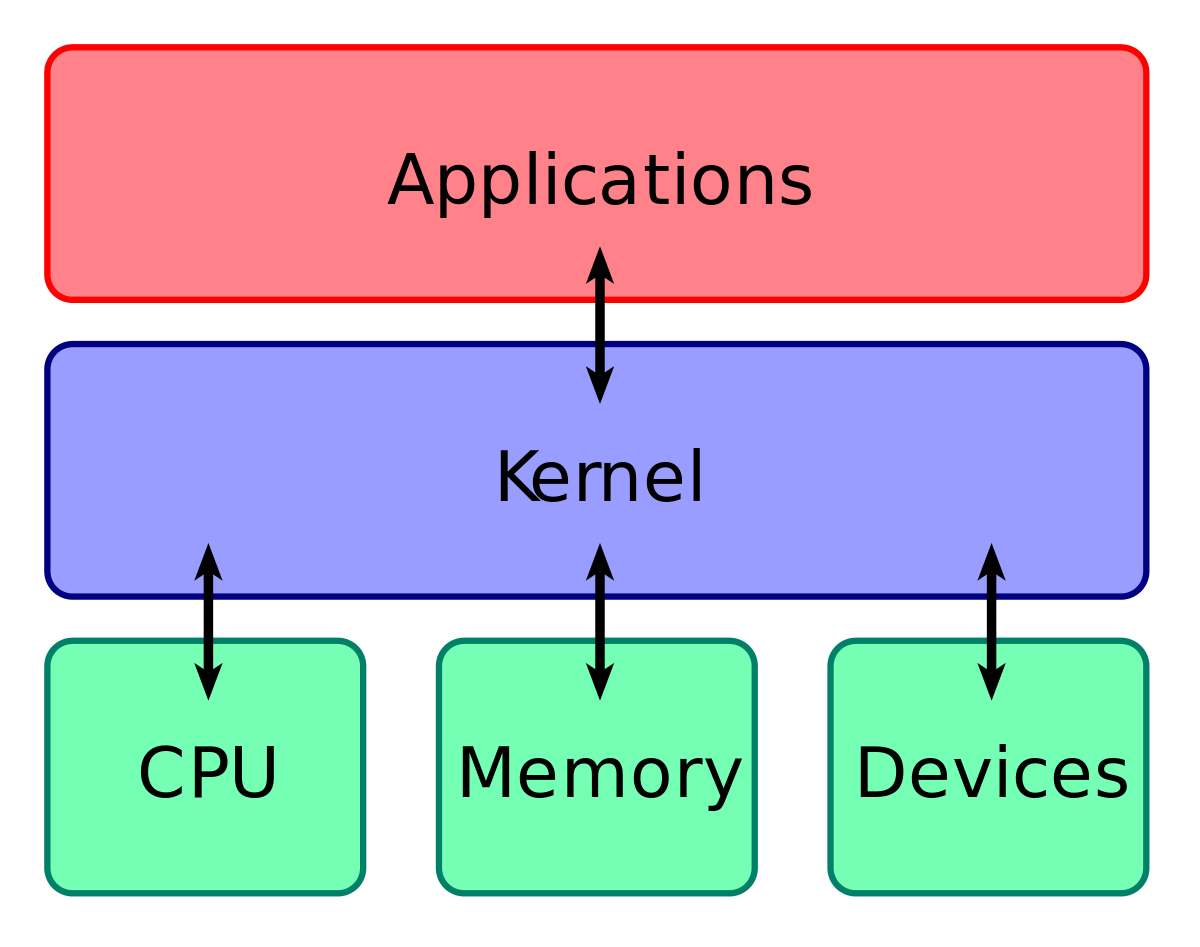
\includegraphics[scale=0.13]{res/Kernel}
    	\end{column}
    \end{columns}
  \end{frame}
  \begin{frame}[fragile]{I moduli del kernel}
    \begin{columns}
    	\begin{column}{0.4\textwidth}
    		\begin{itemize}
    			\item<1> File oggetto caricati e rimossi a runtime
    			\item<2> Estendono le funzionalità del kernel
    		\end{itemize}
    	\end{column}
    	\begin{column}{0.6\textwidth}
    		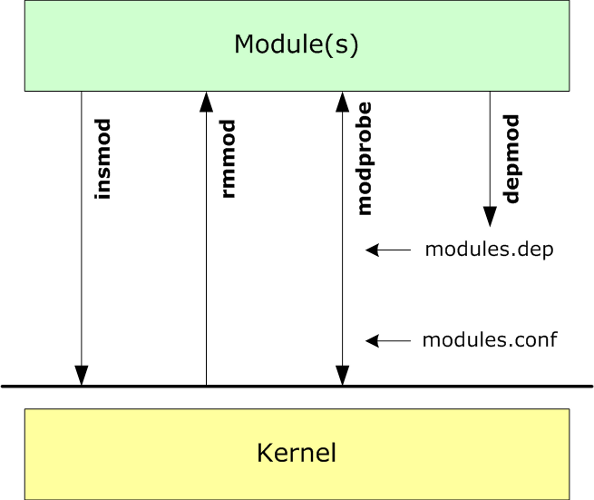
\includegraphics[scale=0.3]{res/Module}
    	\end{column}
    \end{columns}
  \end{frame}
  % ------------------------------------------------------------------------------------------------------------
  %													SPACES
  % ------------------------------------------------------------------------------------------------------------
  \begin{frame}[fragile]{Spazi d'esecuzione}
    \begin{center}
    	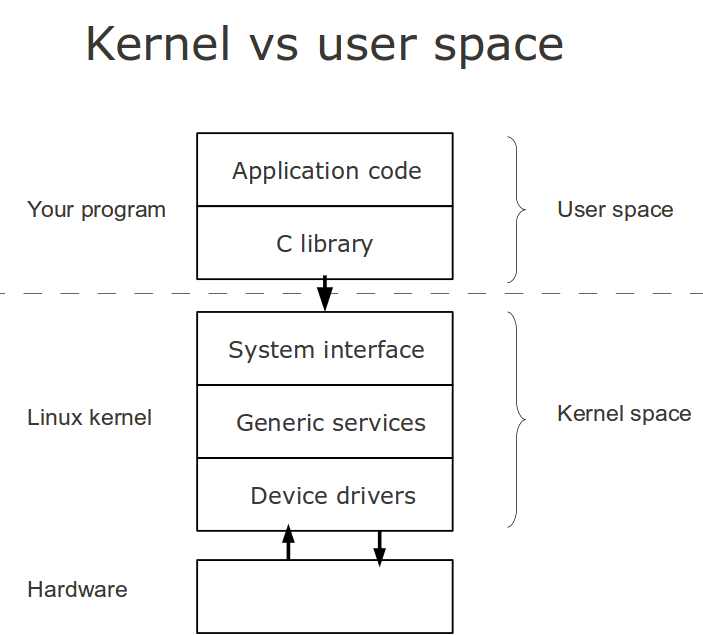
\includegraphics[scale=1.0]{res/Spaces}
    \end{center}
  \end{frame}
  
  % ------------------------------------------------------------------------------------------------------------
  %													SYSCALL
  % ------------------------------------------------------------------------------------------------------------
  \begin{frame}[fragile]{System call}
    \begin{center}
    	Modalità per interagire con il sistema operativo
    	\vfill
    	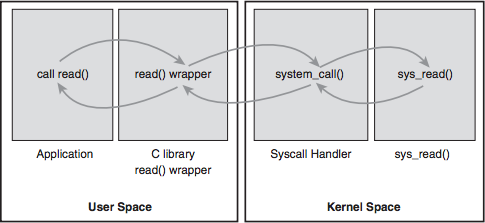
\includegraphics[scale=0.5]{res/Syscall2}
    \end{center}
  \end{frame}

  \section{Linux Kernel Runtime Guardian}
  % ------------------------------------------------------------------------------------------------------------
  %													LKRG
  % ------------------------------------------------------------------------------------------------------------
  \begin{frame}[fragile]{LKRG - Introduzione}
  	\begin{center}
    	È un modulo con l'obiettivo di eseguire controlli d'integrità del kernel e rilevare possibili attacchi di tipo 'exploitation'
    \end{center}
    \begin{center}
    	
\includegraphics[scale=0.10]{res/Lkrg}
    \end{center}
  \end{frame}
  \begin{frame}[fragile]{LKRG - Funzionamento}
    	\begin{columns}
    		\begin{column}{0.5\textwidth}
    			\begin{itemize}
    				\item<1> Salvataggio e confronto degli hash di alcune regioni del sistema
    				\item<2> Monitoraggio di alcune system call
    				\item<3> Routine di validazione a seconda degli eventi scatenati
    			\end{itemize}
    		\end{column}
    		\begin{column}{0.5\textwidth}
    			\only<1>{
    				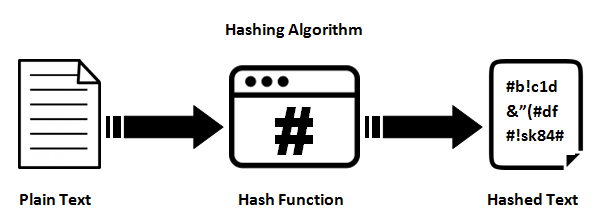
\includegraphics[scale=1.0]{res/Hash}
    			}
    			\only<2>{
    				
\includegraphics[scale=0.45]{res/Intercept}
    			}
    			\only<3>{
    				
\includegraphics[scale=0.2]{res/Routine}
    			}
    		\end{column}
    	\end{columns}
  \end{frame}


  \section{SysBench}
  % ------------------------------------------------------------------------------------------------------------
  %													SYSBENCH
  % ------------------------------------------------------------------------------------------------------------
  \begin{frame}[fragile]{SysBench - Obiettivo}
    \begin{center}
    	Software scritto il linguaggio C al fine di misurare il tempo d'esecuzione di alcune system call monitorate dal Linux Kernel Runtime Guardian
    \end{center}
    \begin{center}
    	
\includegraphics[scale=0.15]{res/Stopwatch}
    \end{center}
  \end{frame}
  \begin{frame}[fragile]{SysBench - Architettura}
    \begin{center}
    	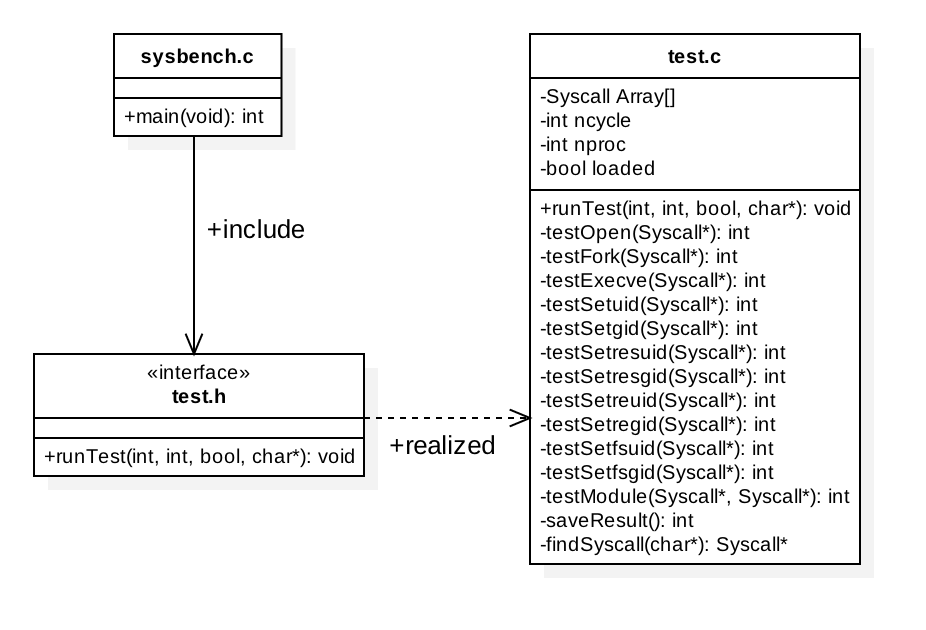
\includegraphics[scale=0.3]{res/Architecture}
    \end{center}
  \end{frame}
  \begin{frame}[fragile]{SysBench - Caso d'uso}
    \begin{center}
    	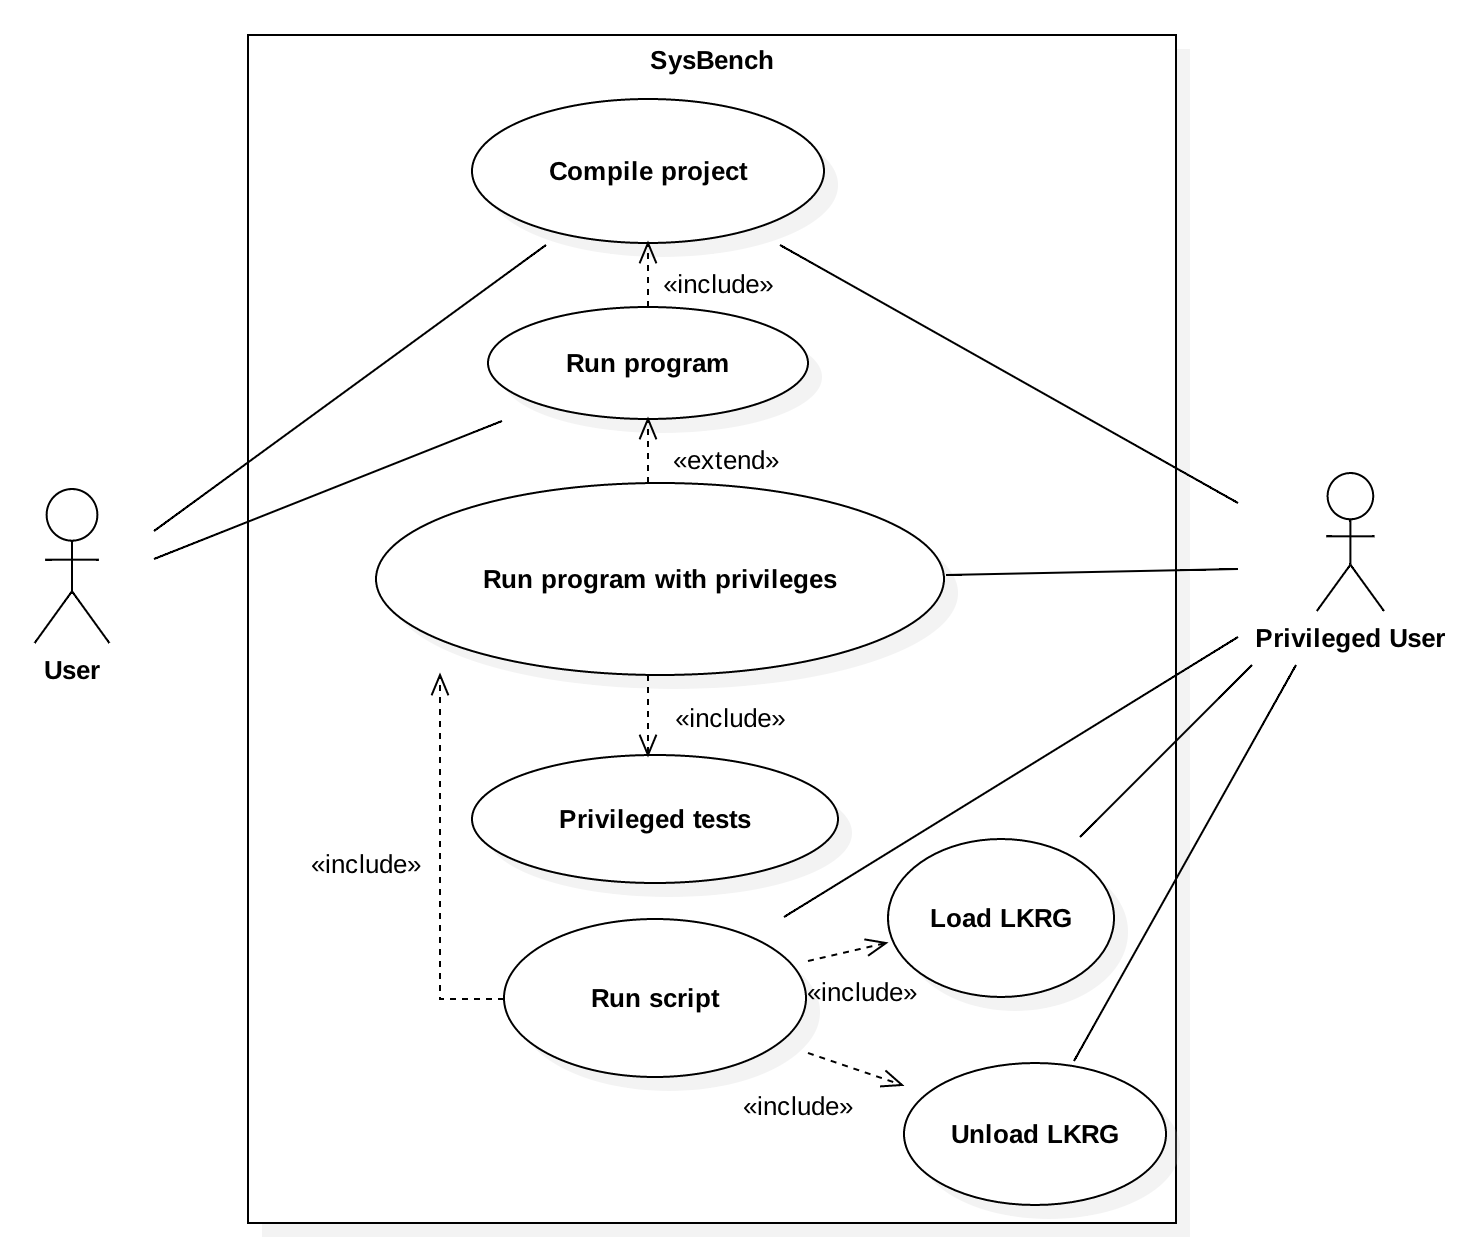
\includegraphics[scale=0.18]{res/UseCase}
    \end{center}
  \end{frame}



  \section{Analisi dei risultati ottenuti}
  % ------------------------------------------------------------------------------------------------------------
  %													ANALYSIS
  % ------------------------------------------------------------------------------------------------------------
  \begin{frame}[fragile]{Analisi - Informazioni dei sistemi}
    \begin{center}
    	Host macOs High Sierra\\
    	
\includegraphics[scale=0.15]{res/Apple}\\
    	Guests Linux\\
    	\begin{tabular}{ c c c }
    		
\includegraphics[scale=0.14]{res/Ubuntu} &
    		
\includegraphics[scale=0.2]{res/Debian} & 
    		
\includegraphics[scale=0.15]{res/Mint} \\
    		Ubuntu & Debian & Mint\\
    	\end{tabular}
    \end{center}
  \end{frame}
  \begingroup
  \setlength{\tabcolsep}{4pt}
  \renewcommand{\arraystretch}{1.5}
  \begin{frame}[fragile]{Analisi - Test in Ubuntu}
    \begin{tabular}{ c c }
    	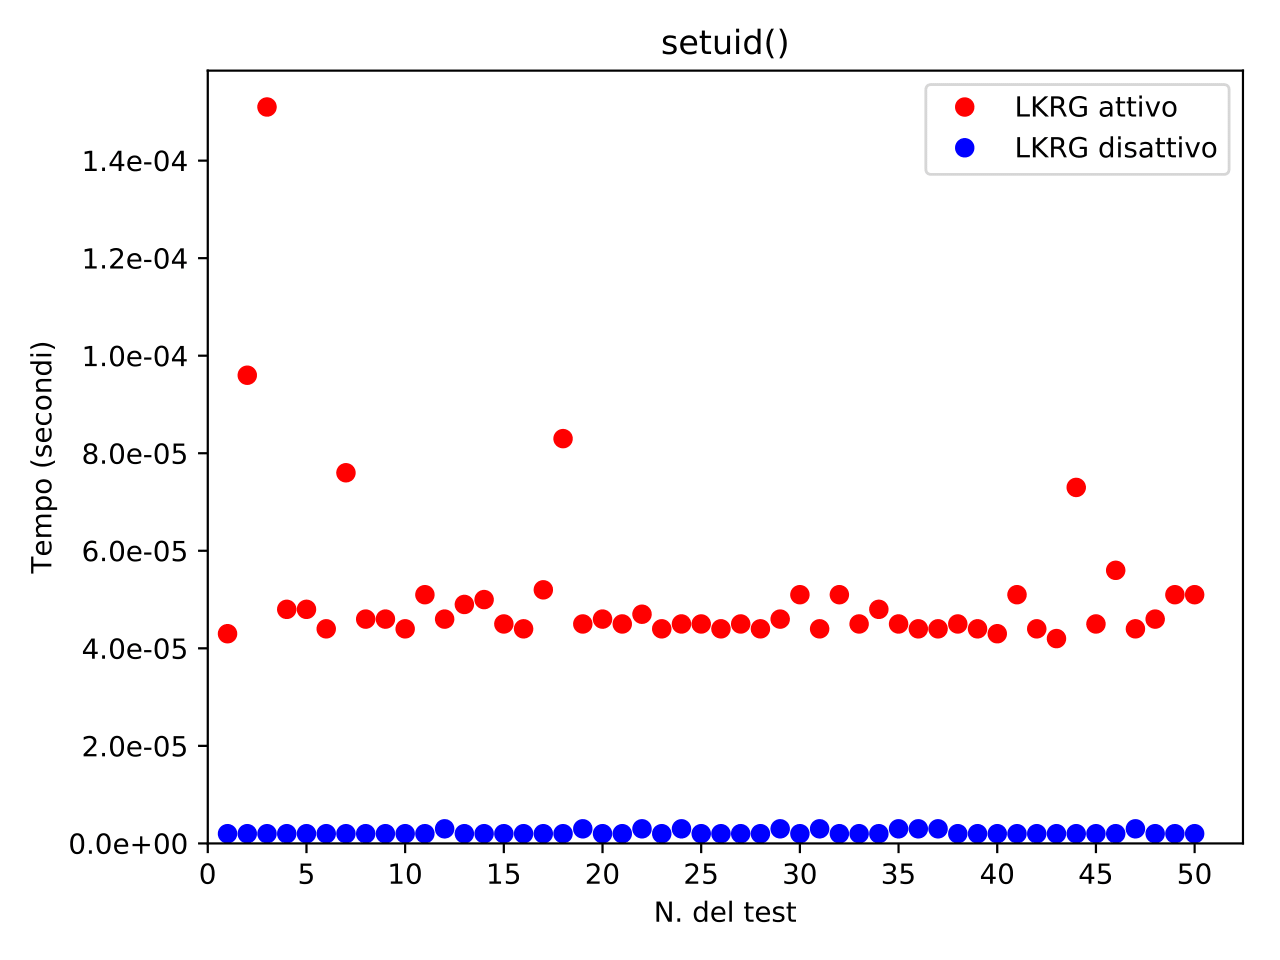
\includegraphics[scale=0.11]{res/Ubuntu/Setuid} & 
    	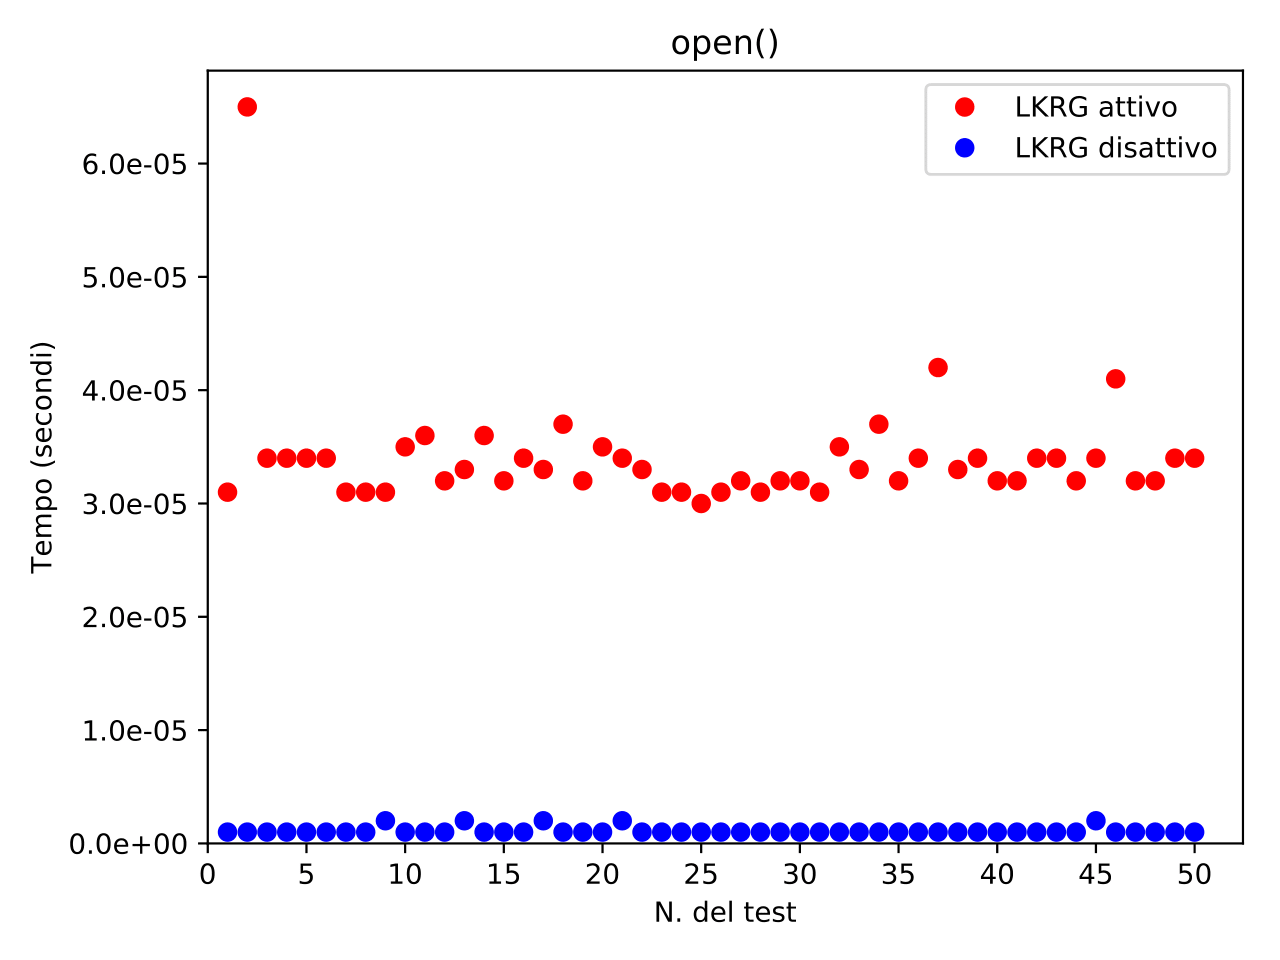
\includegraphics[scale=0.11]{res/Ubuntu/Open}\\
    	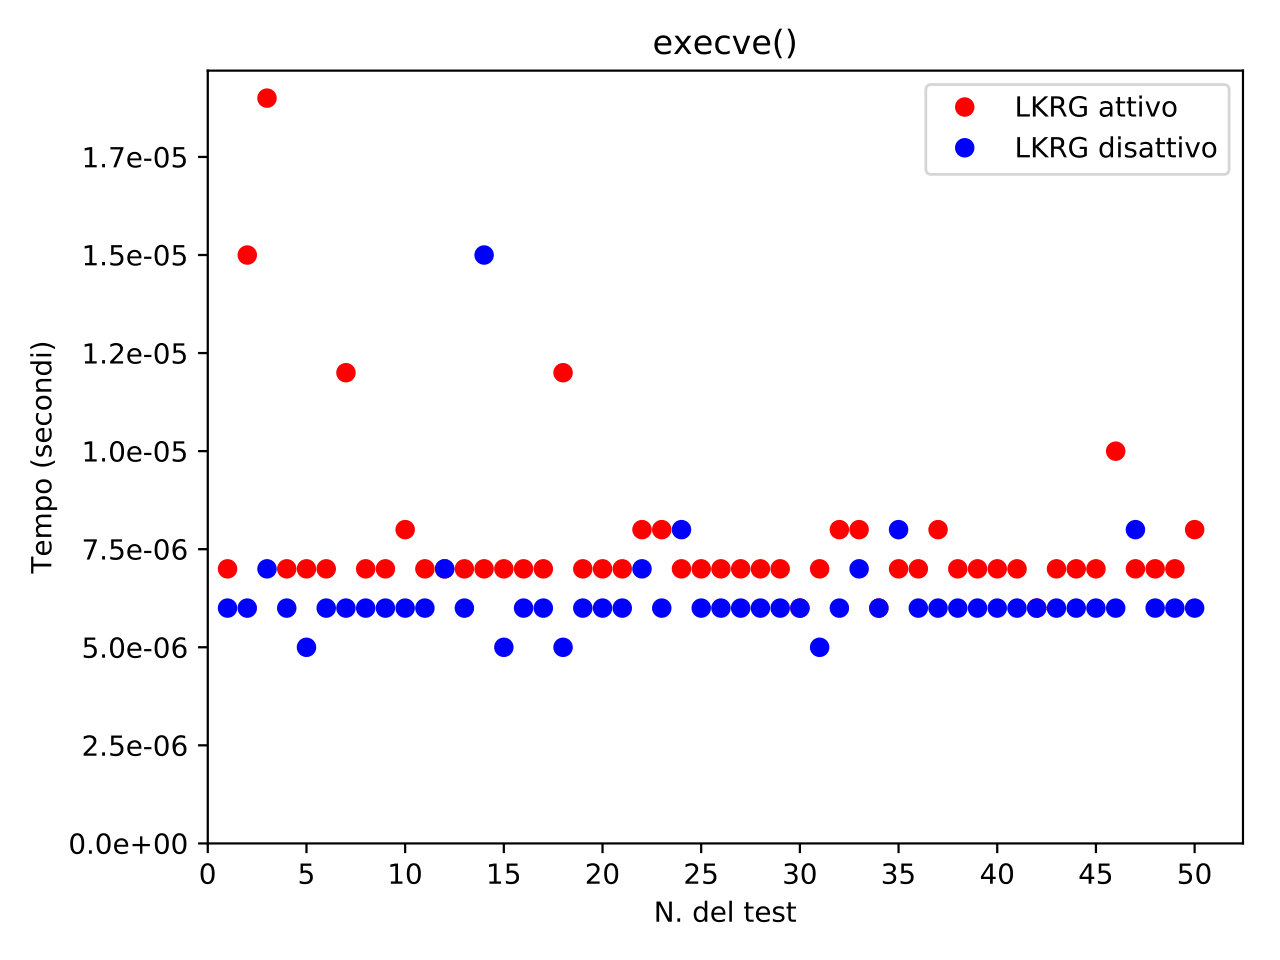
\includegraphics[scale=0.11]{res/Ubuntu/Execve} & 
    	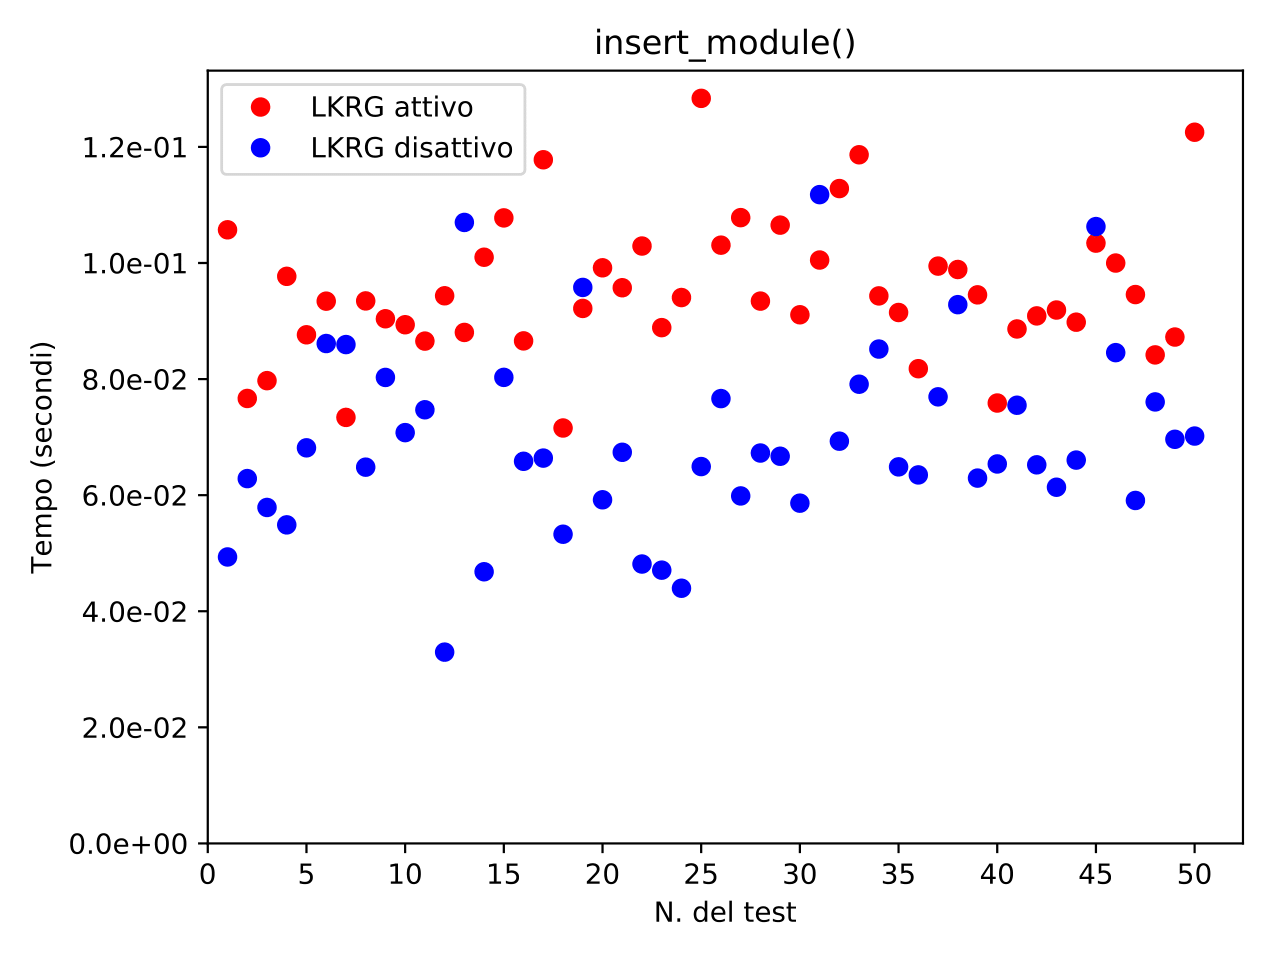
\includegraphics[scale=0.11]{res/Ubuntu/Insert} \\
    \end{tabular}
  \end{frame}
  \begin{frame}[fragile]{Analisi - Test in Debian}
  	\begin{tabular}{ c c }
    	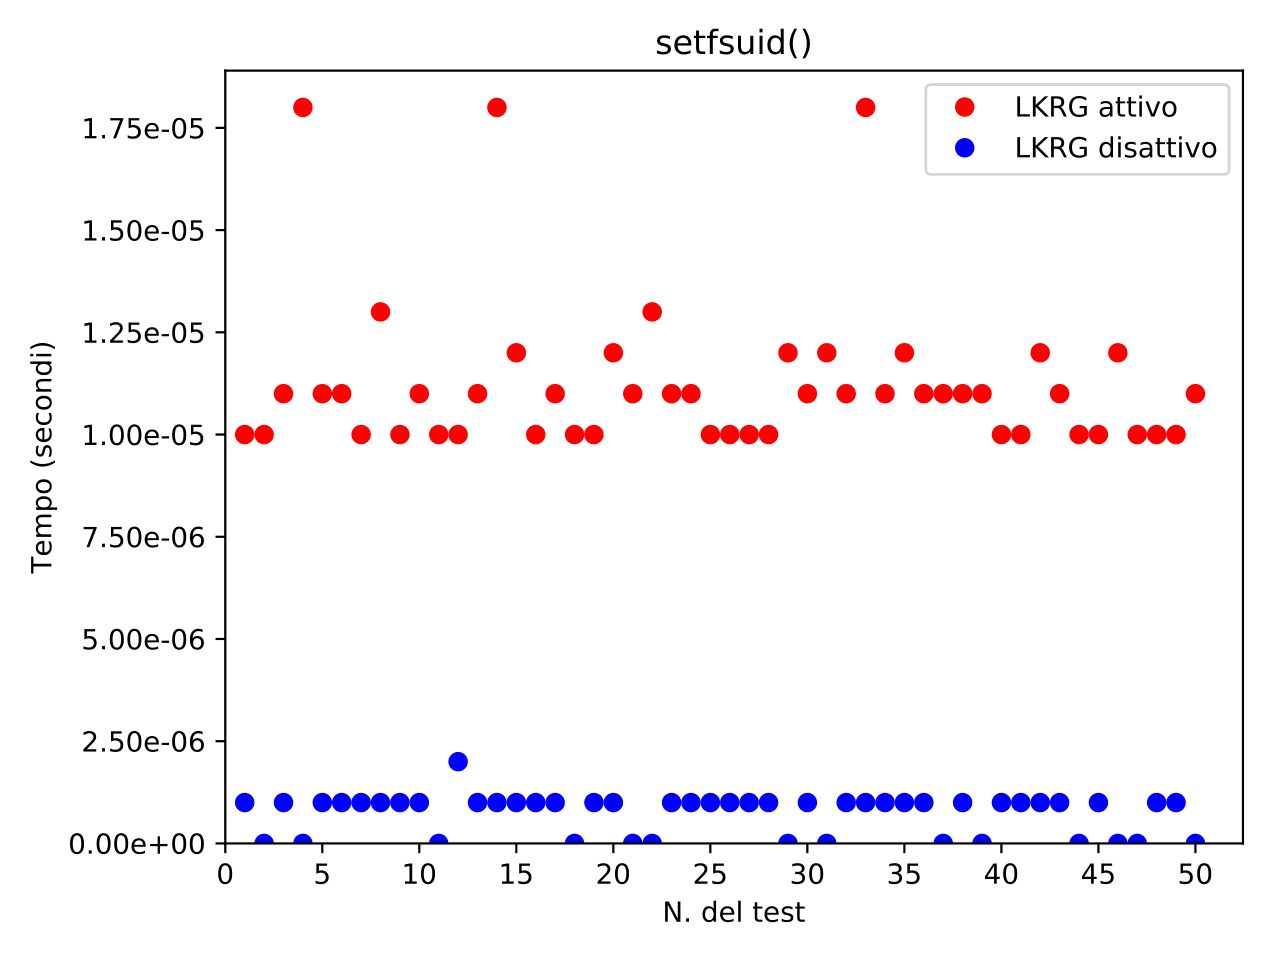
\includegraphics[scale=0.11]{res/Debian/Setfsuid} & 
    	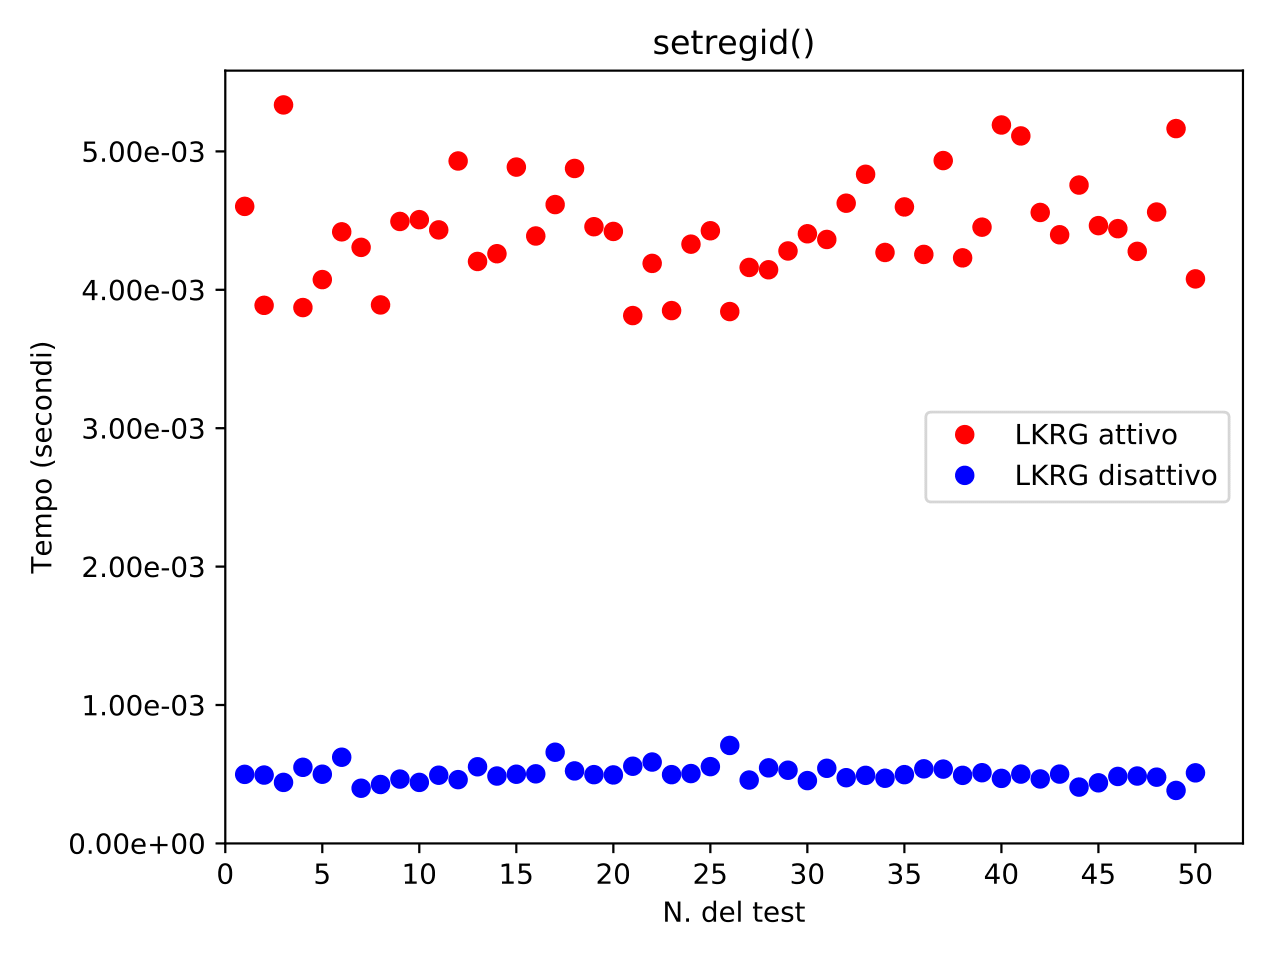
\includegraphics[scale=0.11]{res/Debian/Setregid}\\
    	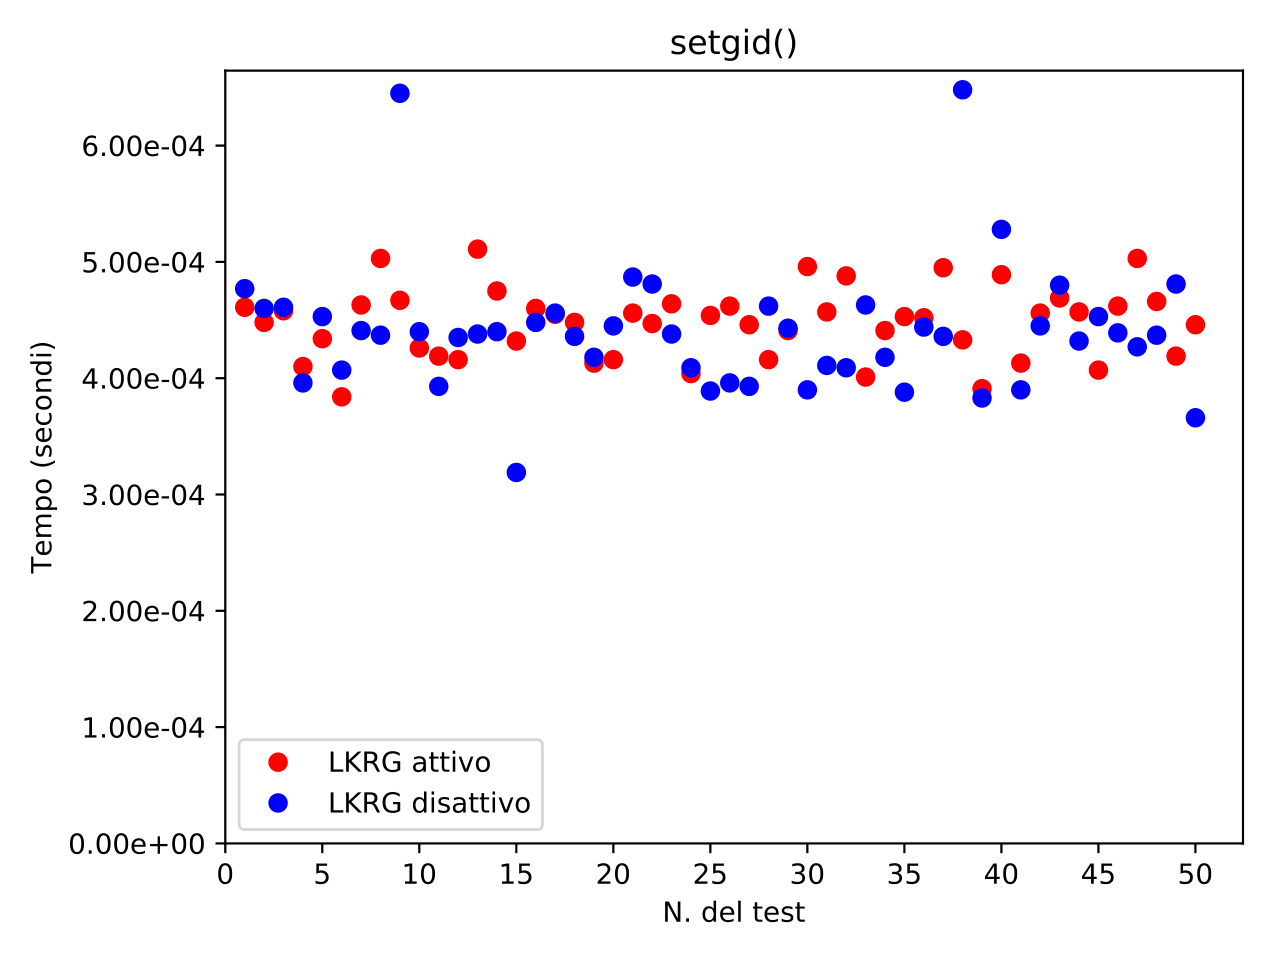
\includegraphics[scale=0.11]{res/Debian/Setgid} & 
    	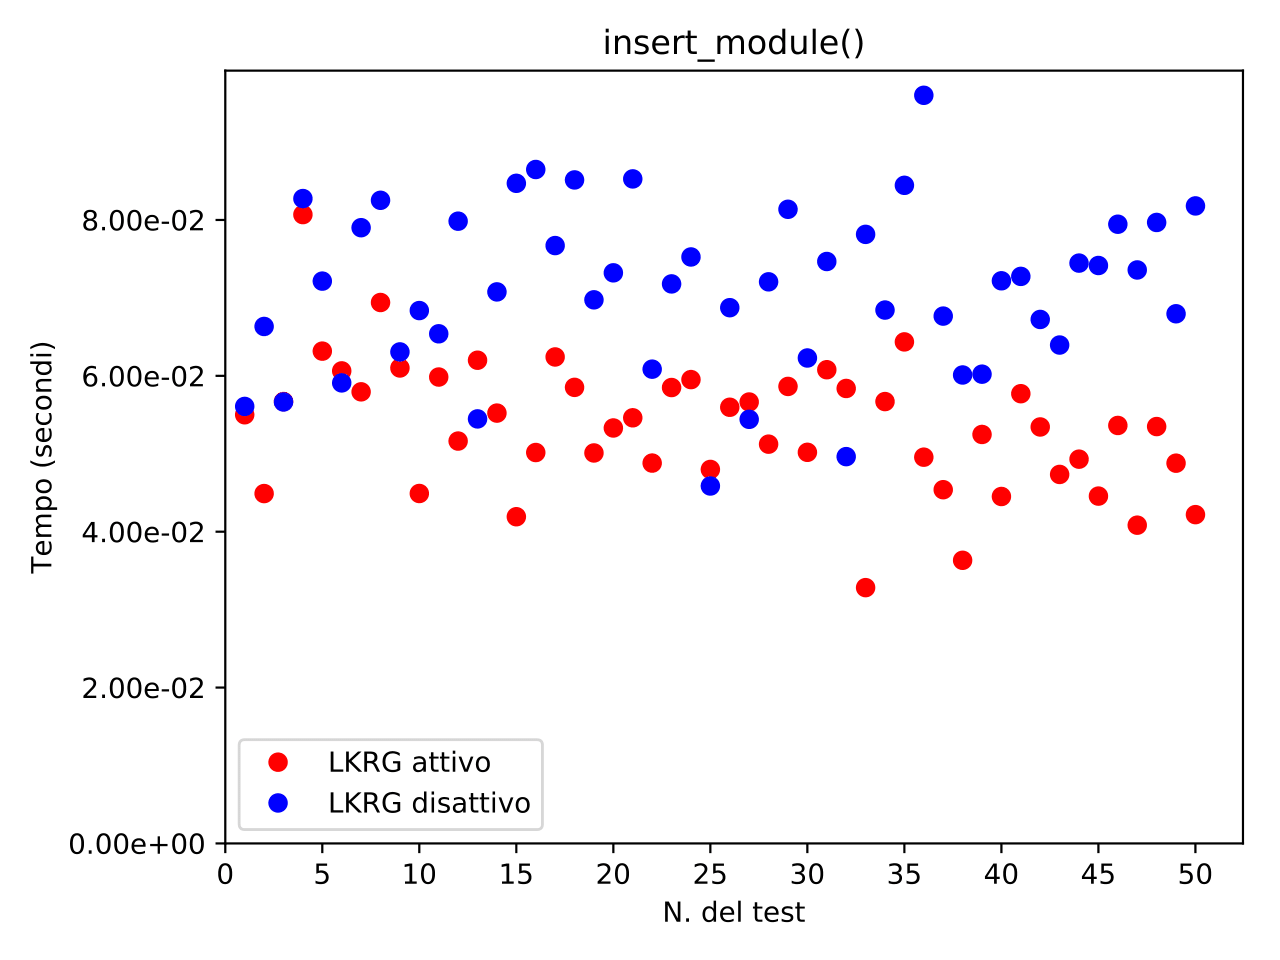
\includegraphics[scale=0.11]{res/Debian/Insert}\\
    \end{tabular}
  \end{frame}
  \begin{frame}[fragile]{Analisi - Test in Mint}
  	\begin{tabular}{ c c }
    	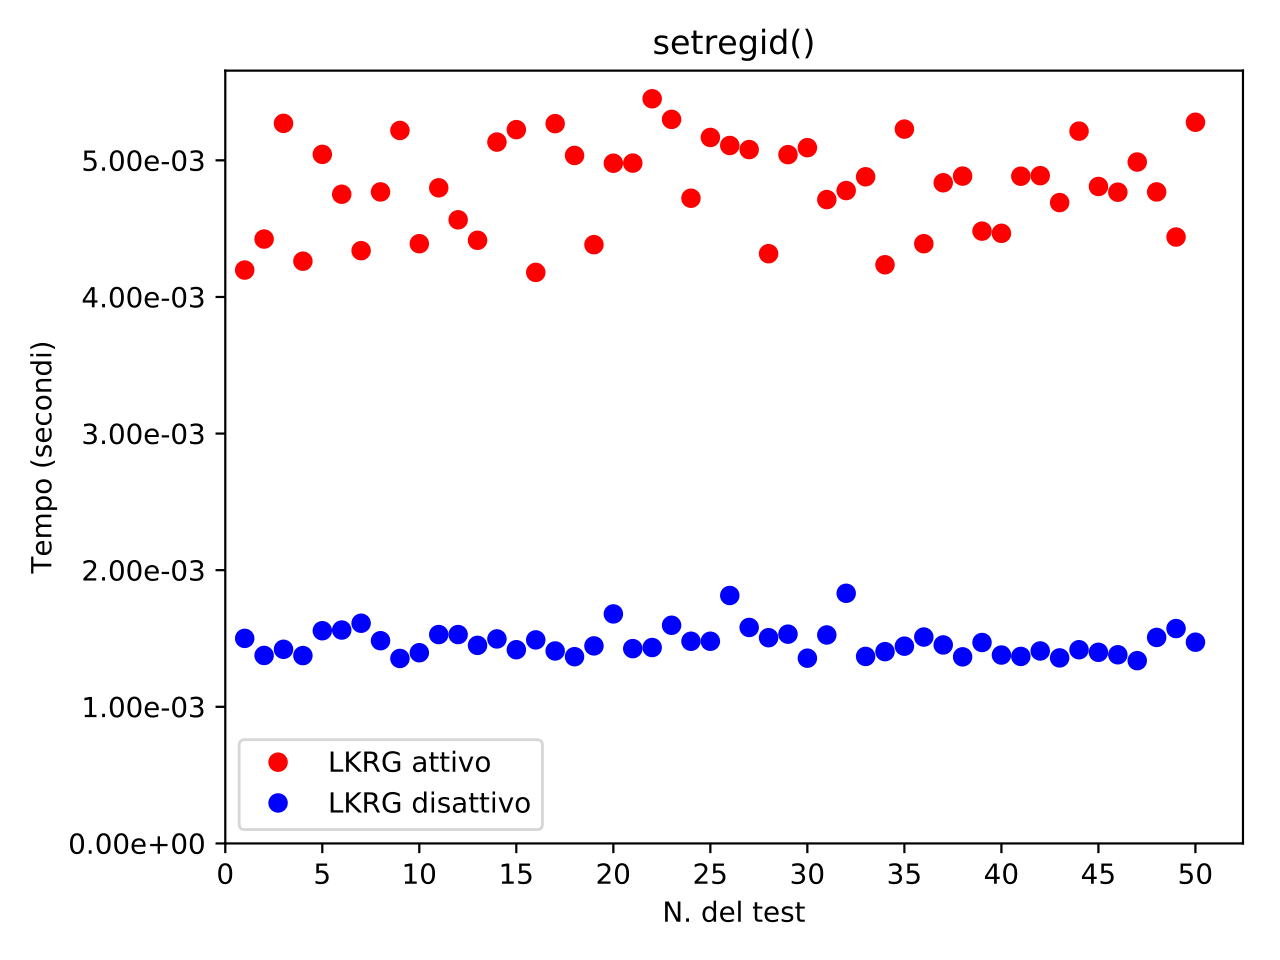
\includegraphics[scale=0.11]{res/Mint/Setregid} &
    	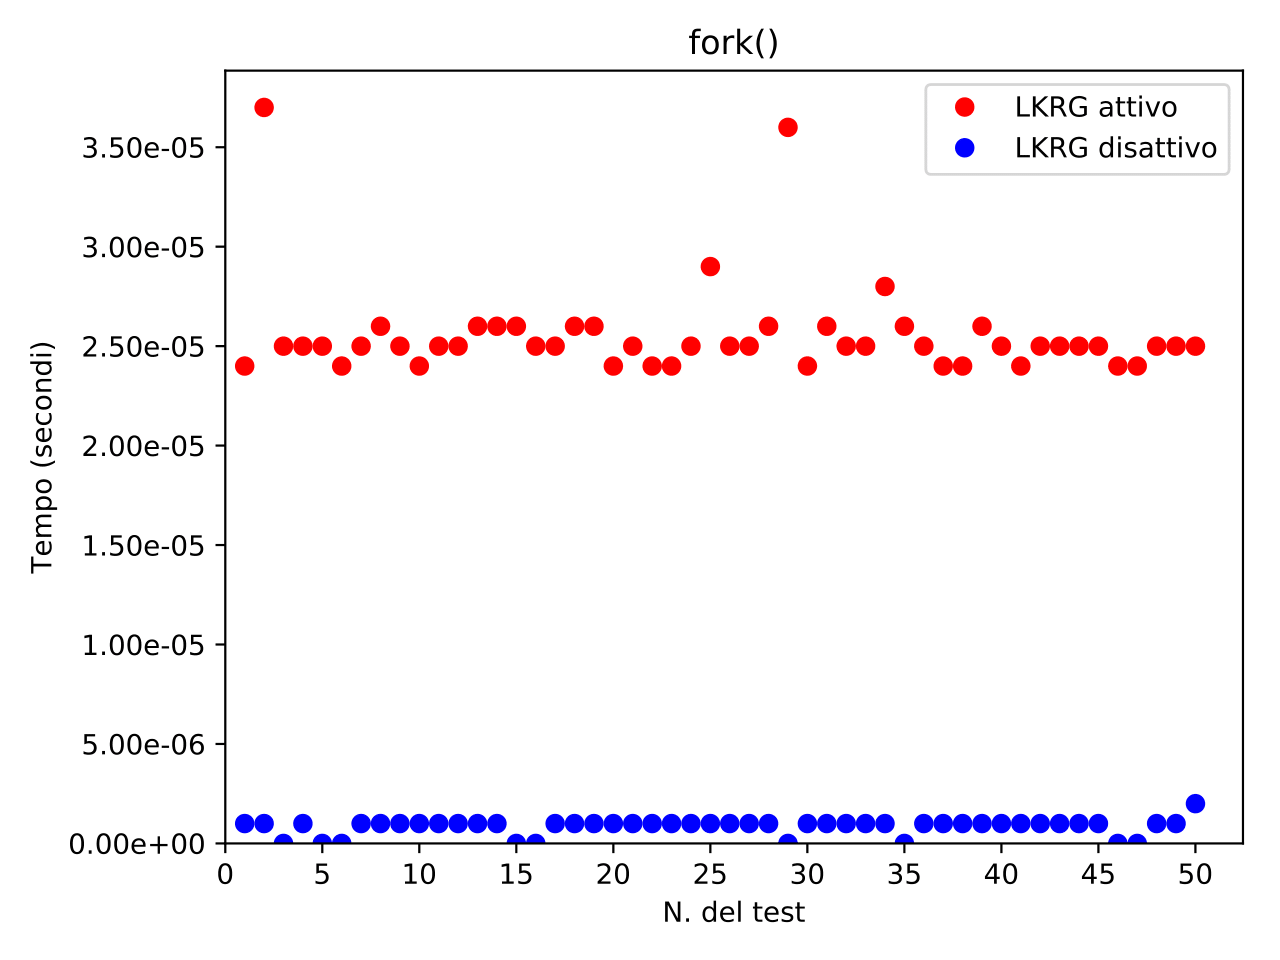
\includegraphics[scale=0.11]{res/Mint/Fork}\\
    	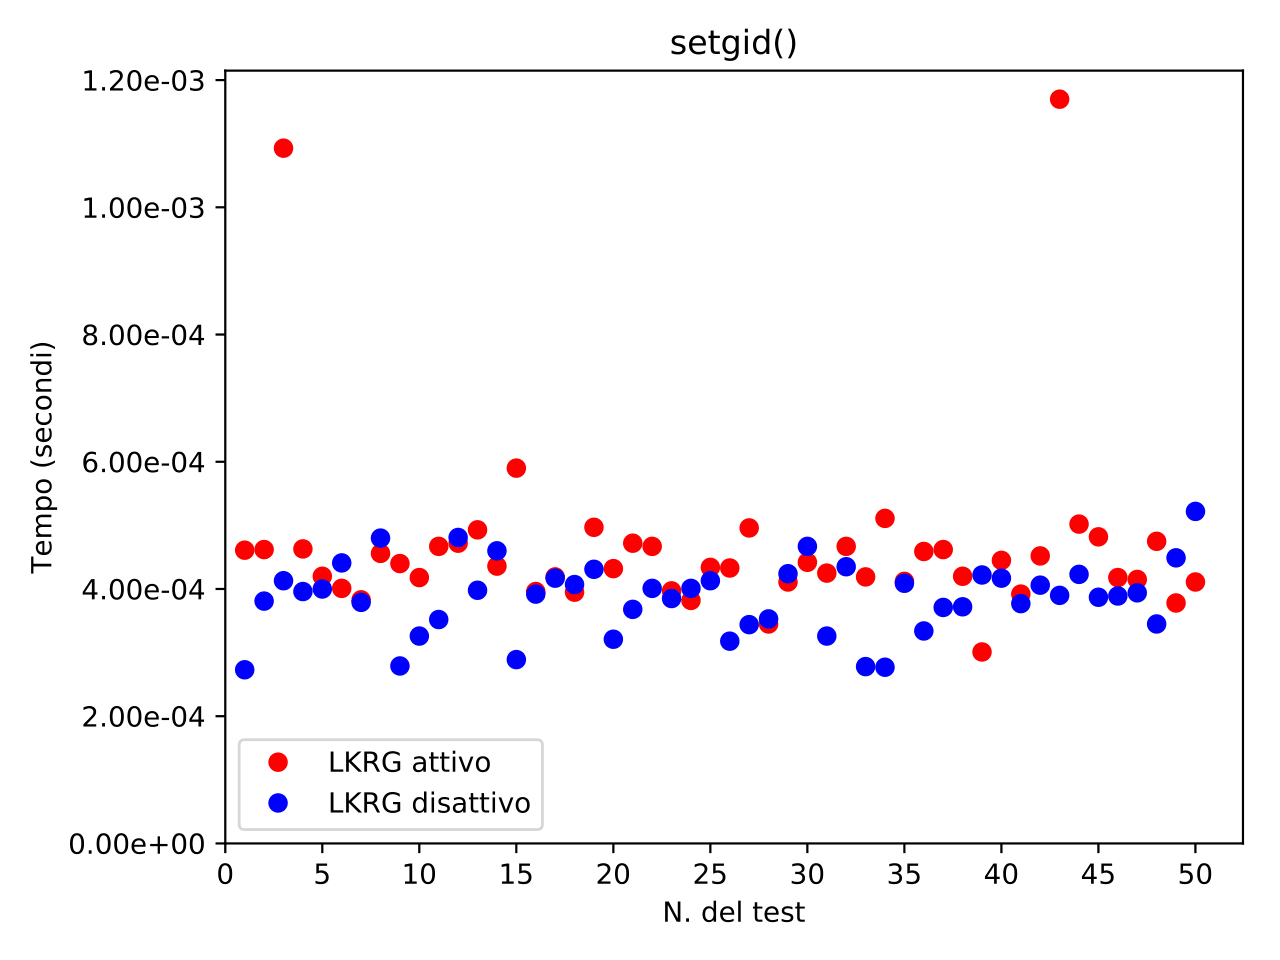
\includegraphics[scale=0.11]{res/Mint/Setgid} & 
    	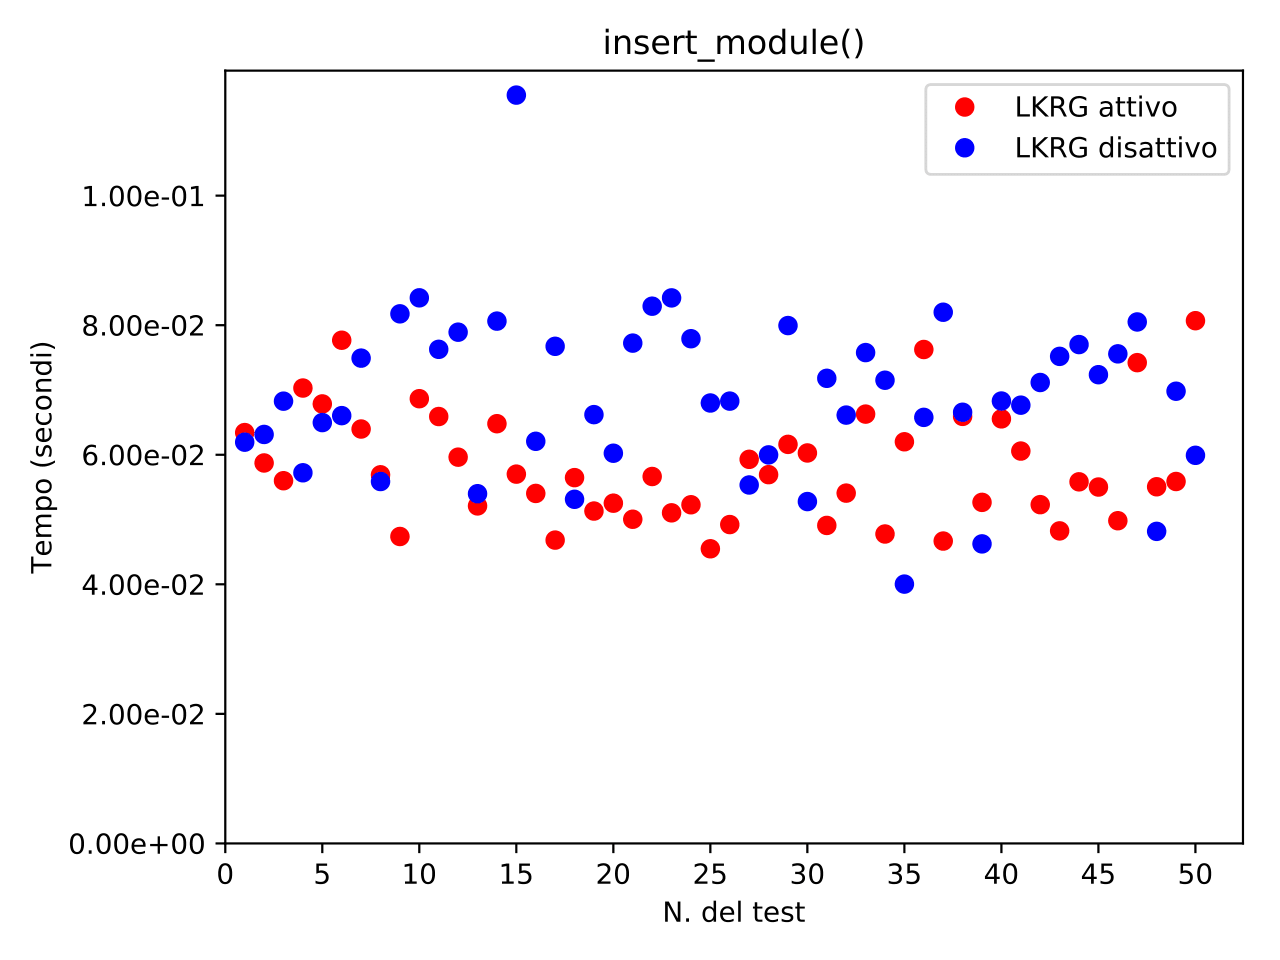
\includegraphics[scale=0.11]{res/Mint/Insert}\\
    \end{tabular}
  \end{frame}
  \endgroup
  \begin{frame}[fragile]{Analisi - Sistemi a confronto}
  	\begin{center}
  		\footnotesize
    	\begin{tabular}{|c|c|c|c|c|}
			\hline
			\textbf{SystemCall} & \bm{$\Delta$}\textbf{ Ubuntu (\%)} & \bm{$\Delta$}\textbf{ Debian (\%)} & \bm{$\Delta$}\textbf{Mint (\%)} \\
			\hline
			setuid() & 2332 & 2193 & 1875 \\
			\hline
			setgid() & 213 & 102 & 121 \\
			\hline
			setresuid() & 3659 & 735 & 2328 \\
			\hline
			setresgid() & 296 & 1597 & 365 \\
			\hline
			setreuid() & 3144 & 1478 & 2136 \\
			\hline
			setregid() & 283 & 884 & 327 \\
			\hline
			setfsuid() & 3406 & 1519 & 3347 \\
			\hline
			setfsgid() & 3824 & 1861 & 4746 \\
			\hline
			open() & 3089 & 1978 & 3051 \\
			\hline
			fork() & 2792 & 1906 & 3043 \\
			\hline
			execve() & 123 & 143 & 115 \\
			\hline
			insert\_module() & 137 & 75 & 84 \\
			\hline
			delete\_module() & 3432 & 1411 & 3581 \\
			\hline
			\hline
			Media & 2056 & 1222 & 1932 \\
			\hline
		\end{tabular}
    \end{center}
  \end{frame}
  \begin{frame}[fragile]{Analisi - Ottimizzazioni}
    \begin{columns}
    		\begin{column}{0.4\textwidth}
    			\begin{itemize}
    				\item<1> Influenza rilevante di LKRG
    				\item<2> Influenza irrilevante di LKRG
    			\end{itemize}
    		\end{column}
    		\begin{column}{0.7\textwidth}
        \begin{overprint}
        \begin{center}
    			\only<1>{
    				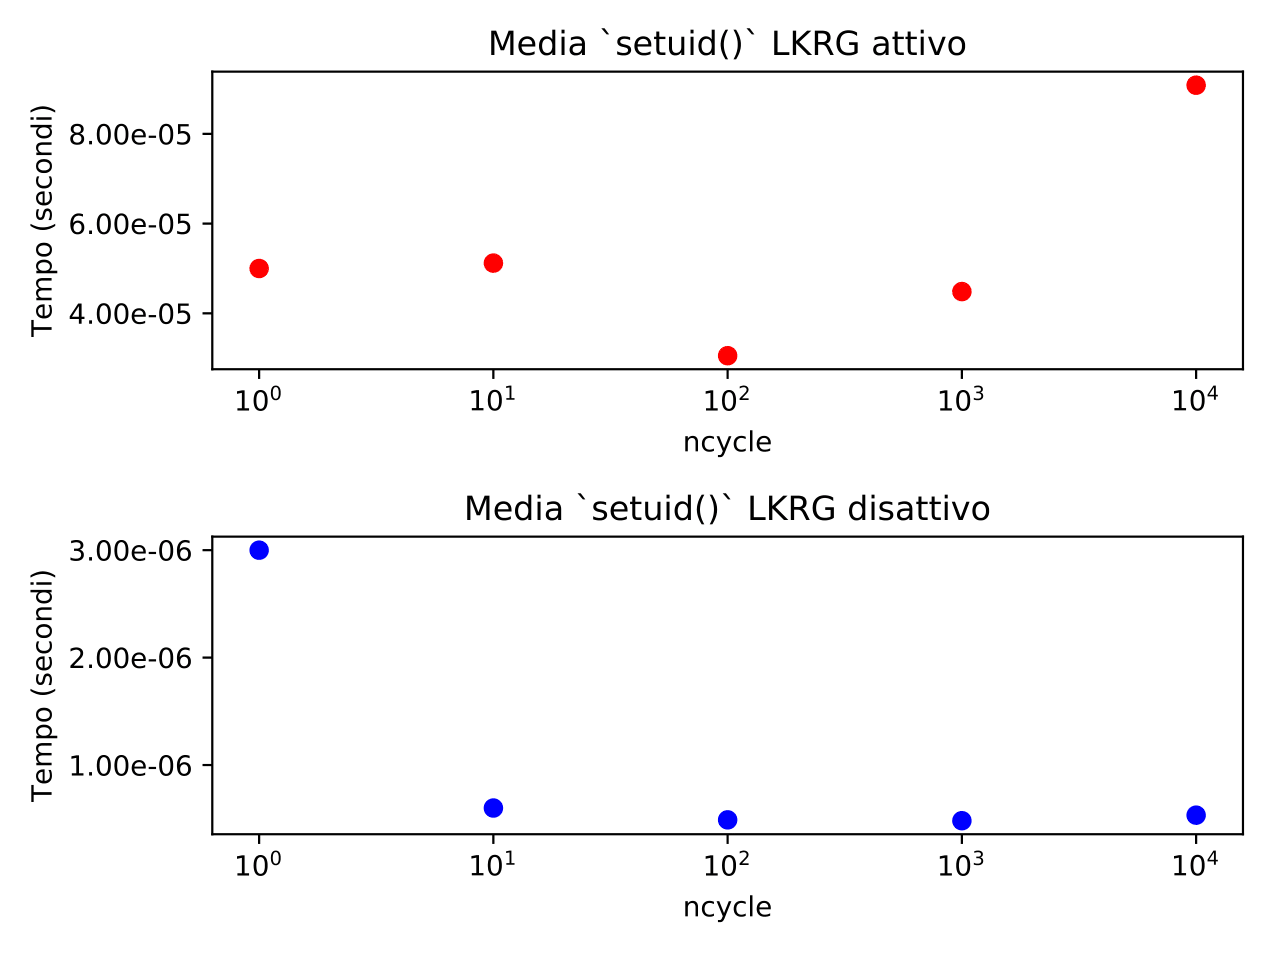
\includegraphics[scale=0.15]{res/Optimization1}
    			}
    			\only<2>{
    				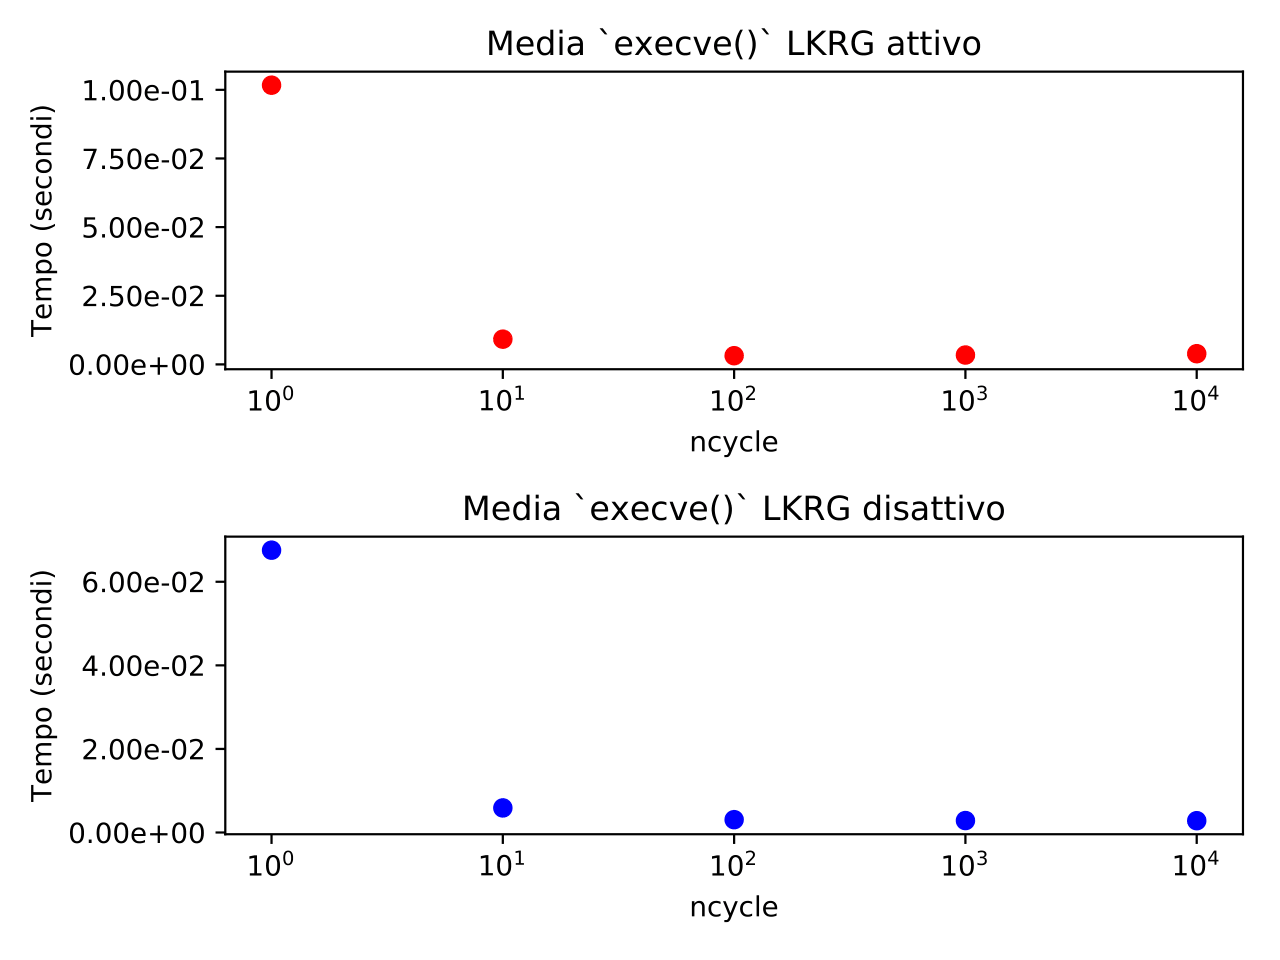
\includegraphics[scale=0.15]{res/Optimization2}
    			}
          \end{center}
          \end{overprint}
    		\end{column}
    	\end{columns}
  \end{frame}

  \section{Conclusioni}
  % ------------------------------------------------------------------------------------------------------------
  %													RINGRAZIAMENTI
  % ------------------------------------------------------------------------------------------------------------
  \begin{frame}[fragile]{Ringraziamenti}
  	Un ringraziamento speciale alle seguenti persone:
  	\begin{columns}
    	\begin{column}{0.7\textwidth}
      		\begin{itemize}
  				\item Gabriele D'Angelo
  				\item Rosanna, Fabrizio e Francesco
  				\item Catarina
  				\item Tutti gli amici più cari
  				\item CeSeNA Security Team
  			\end{itemize}
    	\end{column}
    	\begin{column}{0.4\textwidth}
      		
\includegraphics[scale=0.4]{res/Acknowledgments}
    	\end{column}
  	\end{columns}
  \end{frame}
  % ------------------------------------------------------------------------------------------------------------
  %													END
  % ------------------------------------------------------------------------------------------------------------
  \begin{frame}[standout]
  	FINE\\\vspace{1cm}
  	\begingroup
  		\footnotesize
  		A cura di Simone Magnani\\
  		(~s41m0n~)\\
  		<~simonemagnani.96@gmail.com~>\\[\baselineskip]
  		
\includegraphics[scale=0.17]{res/Linkedin}
  		
\includegraphics[scale=0.05]{res/GitHub}
  		
\includegraphics[scale=0.04]{res/Facebook}
  	\endgroup
\end{frame}
\end{document}